While training and testing in simulated environments offers a fast and safe way to develop algorithms, real-world deployment often reveals significant discrepancies. This is known as \textbf{Sim2Real} gap. The discrepancies arise from the fact that simulations typically use idealized or simplified models of the environment and the robot. In reality, factors like sensor noise, unmodeled dynamics, imperfect actuators, environmental variabilities and physical wear are present.

Bridging this gap is crucial for deploying AI systems in robotics, as the algorithms need to generalize to new, unseen real-world conditions, especially in environments where real-world data is limited or too costly to acquire. Typical strategies include \textit{domain randomization} or \textit{domain adaptation}.

\subsection{Domain Randomization}
\label{subsec:domain-randomization}

\begin{figure}[h]
	\centering
	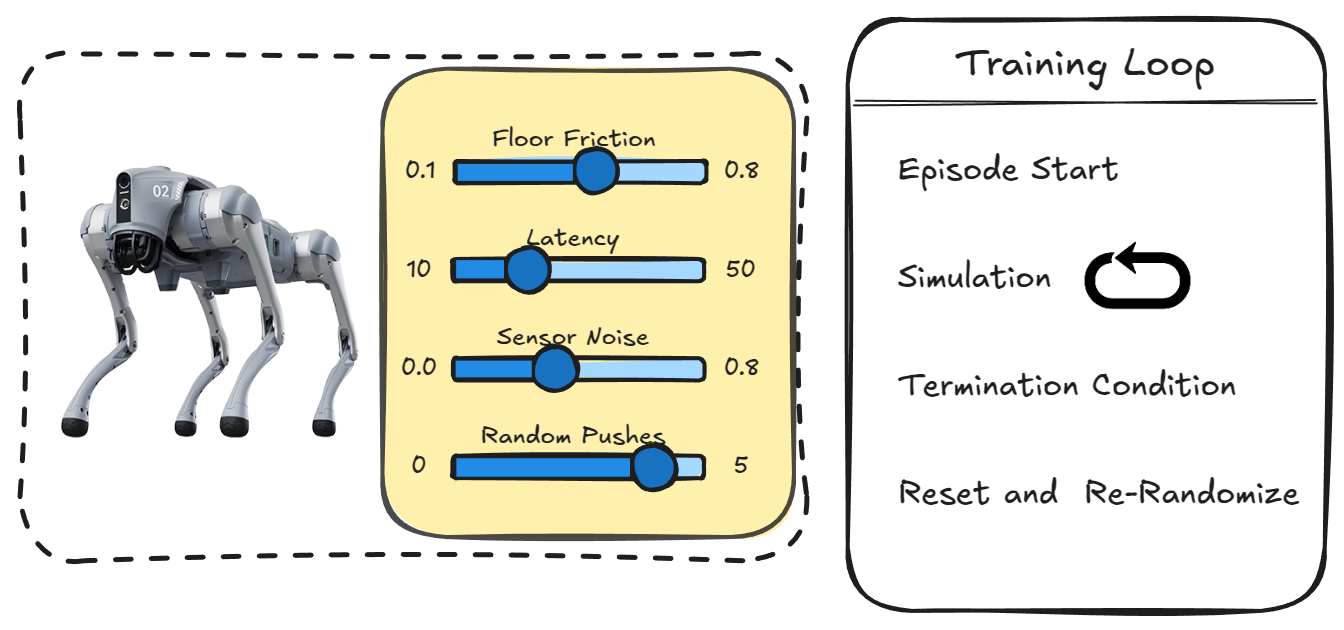
\includegraphics[width=0.8\textwidth]{fig/domain-randomization}
	\caption{Domain Randomization: Introducing random variations in the simulation environment to improve generalization.}
	\label{fig:domain-randomization}
\end{figure}

Instead of performing time-consuming and expensive system identification or gathering extensive real-world data, domain randomization deliberately introduces random variations in the simulated environment's parameters during training, allowing us to artificially create a diverse range of simulation environments. This strategy forces the agent to adapt to a broader set of possible conditions, which in turn helps the model generalize better to real-world scenarios, where conditions may vary due to factors like friction, mechanical noise, etc.

Several parameters in the simulation can be randomized, including:

\begin{itemize}
	\item \textbf{Floor Friction}: Varying the coefficient of friction on surfaces simulates different floor types, weather conditions, or wear on the robot's legs. This allows the robot to learn strategies that adapt to a variety of environments.
	
	\item \textbf{Latency}: By randomly adjusting communication delays or actuator response times in the simulation, the robot can learn to handle real-world delays that may affect its control strategies.
	
	\item \textbf{Physical Parameters}: Modifying parameters such as mass, inertia, battery voltage, and motor friction helps the model account for real-world variations in these key aspects of the robot's physical characteristics.
	
	\item \textbf{Sensor Noise}: Introducing random noise to sensory inputs mimics imperfections in real-world sensors, enabling the robot to better handle noisy or imprecise data during operation.
	
	\item \textbf{Forces}: Applying random forces during the simulation makes the robot robust against external forces (ex: someone pushes or pulls the robot).
\end{itemize}

Basically, in training, every time there is a termination condition and the episode is reset, besides re-initializing the initial pose and velocities of the robot, there will be a re-initialization accounting also for domain randomization:

\begin{pythoncode}
	# Perform randomization
	env_friction = np.random.uniform(self.min_env_friction, self.max_env_friction)   
	latency = np.random.uniform(self.min_latency, self.max_latency)      
	mass = np.random.uniform(self.min_mass, self.max_mass)        
	IMU_bias = np.random.uniform(self.min_IMU_bias, self.max_IMU_bias) 
	IMU_std = np.random.uniform(self.min_IMU_std, self.max_IMU_std) 
	ext_force = generate_random_force(modulus, direction, duration)
\end{pythoncode}

By using domain randomization, robotic systems become more adaptable to the real world, and can handle scenarios that they were never directly trained on in simulation. However, a limitation of this approach is that the robot will learn a conservative policy able to generalize on different scenarios, rather than an optimal one tailored to specific conditions.

\subsection{Adaptation Strategies}

To improve the generalization of the robot across various environments, the policy can be conditioned on environment parameters ($\mu$). By doing so, the robot can adjust its actions based on both its internal state and the dynamics of the environment. However, in real-world scenarios, these environment parameters are not precisely known. If they were, the problem would already be solved.

\begin{figure}[h]
	\centering
	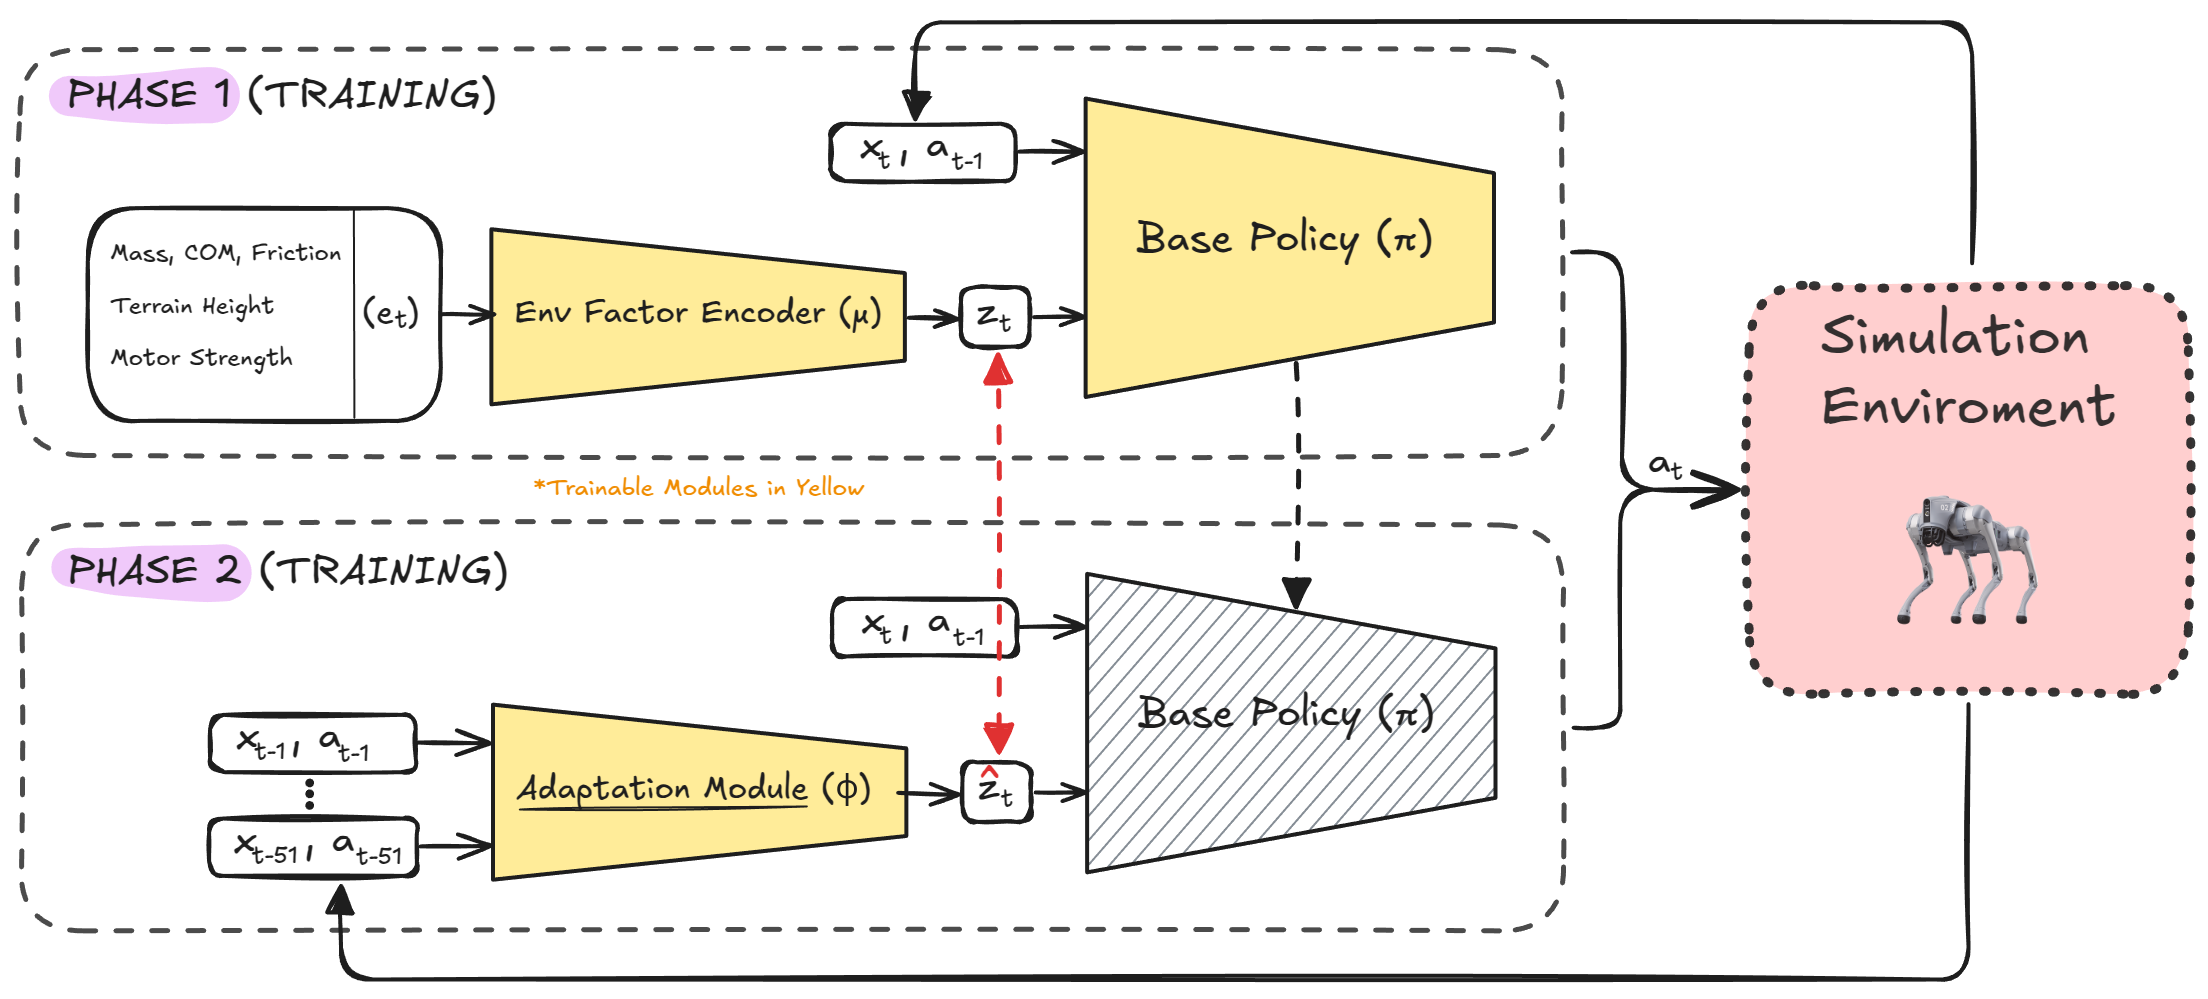
\includegraphics[width=0.8\textwidth]{fig/domain-adaptation-training}
	\caption{Training Pipeline for Domain Adaptation. Phase 1: Environment parameters $\mu$ are encoded into latent $z$ to train the policy $\pi$. Phase 2: The adaptation module $\phi$ learns to estimate $z$ from state/action history. Both phases are trained jointly in simulation using reinforcement learning.}
	\label{fig:training-pipeline}
\end{figure}

\subsubsection{Latent Representation of Environment Parameters}

Fortunately, in simulation, the environment parameters are fully available. In this way, at the beginning of each training episode, a random set of environment parameters $\mu$ is sampled according to a probability distribution $p(\mu)$. These parameters can include friction, latency, sensor noise and other factors that influence the dynamics. Predicting the exact system parameters $\mu$ is often unnecessary and impractical, as it may lead to overfitting and poor real-world performance. Instead, a low-dimensional latent embedding $z$ is used. Once $\mu$ is sampled, the environment parameters are encoded into a compact latent space $z$ using an encoder function $e$, represented as:
\begin{equation*}
	z_t = e(\mu_t)
\end{equation*}
Here, $z_t$ serves as a concise representation of the environment's dynamics. This latent variable is then fed as an additional input to the robot's policy, enabling it to adapt its actions based on the environment:
\begin{equation*}
	\pi(a_t \mid o_t, z_t)
\end{equation*}
Where:
\begin{itemize}
	\item $a_t$: Action to be taken by the robot.
	\item $o_t$: Observations.
	\item $z_t$: Latent encoding of the environment's dynamics.
\end{itemize}

\subsubsection{Training the Policy}

During training, both the encoder $e$ and policy $\pi$ are jointly optimized using gradient descent based on the reward signals, as a typical reinforcement learning problem.

\subsubsection{Real-World Deployment: Adaptation Module}

\begin{figure}[h]
	\centering
	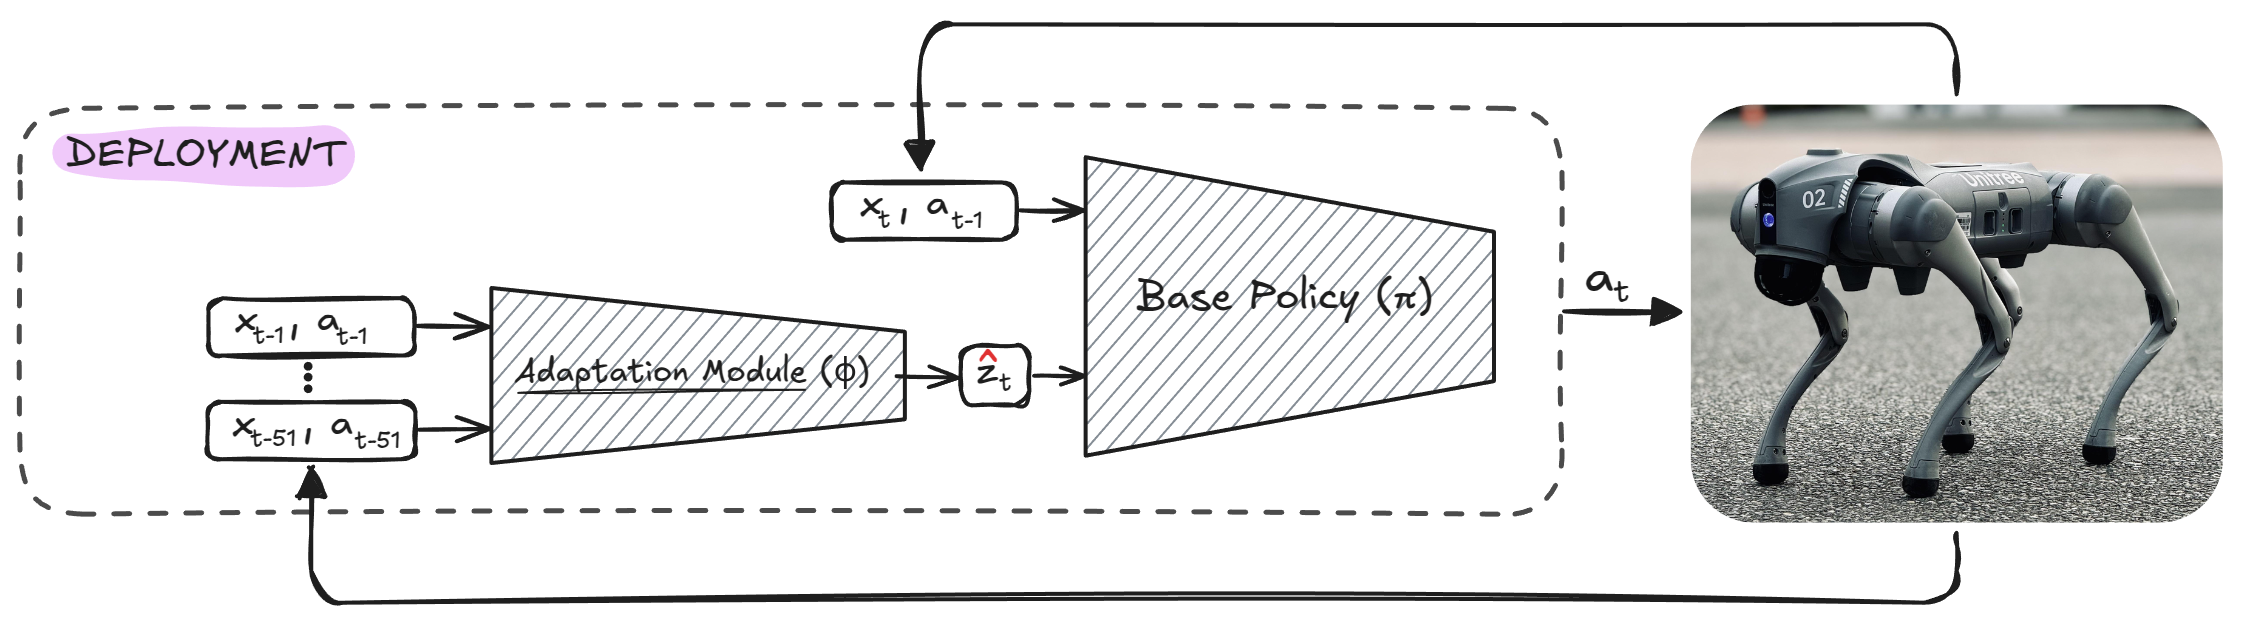
\includegraphics[width=0.8\textwidth]{fig/domain-adaptation-deployment}
	\caption{Real-World Deployment for Domain Adaptation. The adaptation module $\phi$ estimates latent $\hat{z}$ from state/action history, enabling the policy $\pi$ to adapt to real-world conditions without explicit knowledge of environment parameters $\mu$.}
	\label{fig:deployment}
\end{figure}

In real-world deployment, the robot does not have access to the privileged environment parameters $\mu$. Instead, an \emph{adaptation module} ($\phi$) is employed to estimate the latent variable $\hat{z}_t$ online. This estimate is derived from the recent history of the robot's states ($x_{t-k:t-1}$) and actions ($a_{t-k:t-1}$):
\begin{equation}
	\hat{z}_t = \phi(x_{t-k:t-1}, a_{t-k:t-1})
\end{equation}

Unlike traditional system identification approaches that attempt to predict the precise environmental parameters $\mu$, this method directly estimates $\hat{z}_t$.

\subsubsection{Training the Adaptation Module}

The adaptation module $\phi$ is trained in simulation, where both the state-action history and the ground truth extrinsics vector $z_t$ are available. This is a typical supervised learning problem, where the objective is to minimize the \textbf{mean squared error (MSE)} between $\hat{z}_t$ and $z_t$:
\begin{equation}
	\text{MSE}(\hat{z}_t, z_t) = \| \hat{z}_t - z_t \|^2
\end{equation}

This training process ensures that the adaptation module learns to accurately predict $\hat{z}_t$ based on historical data.

\subsubsection{Deployment}

Once trained, the adaptation module and policy are ready for real-world deployment. The policy operates as follows:
\begin{equation}
	\pi(a_t \mid o_t, \hat{z}_t)
\end{equation}

The adaptation module $\phi$ runs asynchronously at a slower frequency, periodically updating $\hat{z}_t$. The policy uses the most recent $\hat{z}_t$ along with the current observations to determine the robot's actions. This design enables robust and efficient performance across diverse real-world environments while maintaining computational efficiency.

\section{Key Works and Citations}
\begin{itemize}
	\item \textbf{Ashish Kumar (2022)}: \href{https://arxiv.org/pdf/2205.15299}{\textit{Adapting Rapid Motor Adaptation for Bipedal Robots}}
	\item \textbf{Ashish Kumar (2021)}: \href{https://arxiv.org/pdf/2107.04034}{\textit{RMA: Rapid Motor Adaptation for Legged Robots}}
	\item \textbf{Xue Bin Peng (2020)}: \href{https://arxiv.org/pdf/2004.00784}{\textit{Learning Agile Robotic Locomotion Skills by Imitating Animals}}
	\item \textbf{Jie Tan (2018)}: \href{https://arxiv.org/pdf/1804.10332}{\textit{Sim-to-Real: Learning Agile Locomotion For Quadruped Robots}}
\end{itemize}
